\subsection{Model Parameter Estimates in the Limit of Large Data Sets} \label{sec:largedata}

The individual \MAP{}s in \citet{bov13} contained typically between 100 and 800 objects, so that each \MAP{} implied a quite broad \pdf{} for the model parameters $\pmodel{}=\{p_\Phi,p_\text{DF}\}$. Here we explore what happens in the limit of much larger samples for each \MAP{}, say 20,000 objects. As outlined in \S\ref{sec:likelihood} the immediate consequence of larger samples is given by the likelihood normalization requirement, $\log(1+\delta M_\text{tot})\le 1/N_{sample}$, (see Equation \ref{eq:loglikelihood_relerr})), which is the modelling aspect that drives the computing time. This issues aside, we would, however, expect that in the limit of large data sets with vanishing measurement errors the \pdf{}s of the \pmodel{} become Gaussian, with a \pdf{} width (i.e. standard error SE of the Gaussian) that scales as $1/\sqrt{N_\text{sample}}$. Further, we must verify that any bias in the \pdf{} expectation value is considerably less than the error (SE), even for quite large samples.

Using sets of mock data, created according to \S\ref{sec:mockdata} and with our fiducial model for \pmodel{} (see Table \ref{tbl:tests}, Tests \ref{test:sqrtNiso}, \ref{test:isoSph_CLT}, and \ref{test:isoSphFlex}), we verified that \RM{} satisfies all these conditions and expectations. Figure \ref{fig:isoSphFlex_triangleplot} illustrates the joint \pdf{}s of all \pmodel{}. This figure illustrates that the \pdf{} is a multivariate Gaussian that projects into Gaussians when considering the marginalized \pdf{} for all the individual \pmodel{}. Note that some of the parameters are quite covariant, but the level of their actual covariance depends on the choice of the \pmodel{} from which the mock data were drawn. Figure \ref{fig:sqrtNiso} then illustrates that the \pdf{} width, SE, indeed scales as $1/\sqrt{N_\text{sample}}$. Figure \ref{fig:isoSph_CLT} illustrates even more that \RM{} satisfies the central limit theorem. The average parameter estimates from many mock samples with identical underlying \pmodel{} are very close to the input \pmodel{}, and the distribution of the actual parameter estimates are a Gaussian around it. 
%
%%====================================================================
%
%%FIGURE: Triangle plot, shape of likelihood, multi-variate Gaussian
%
%\begin{figure*}
%\centering
%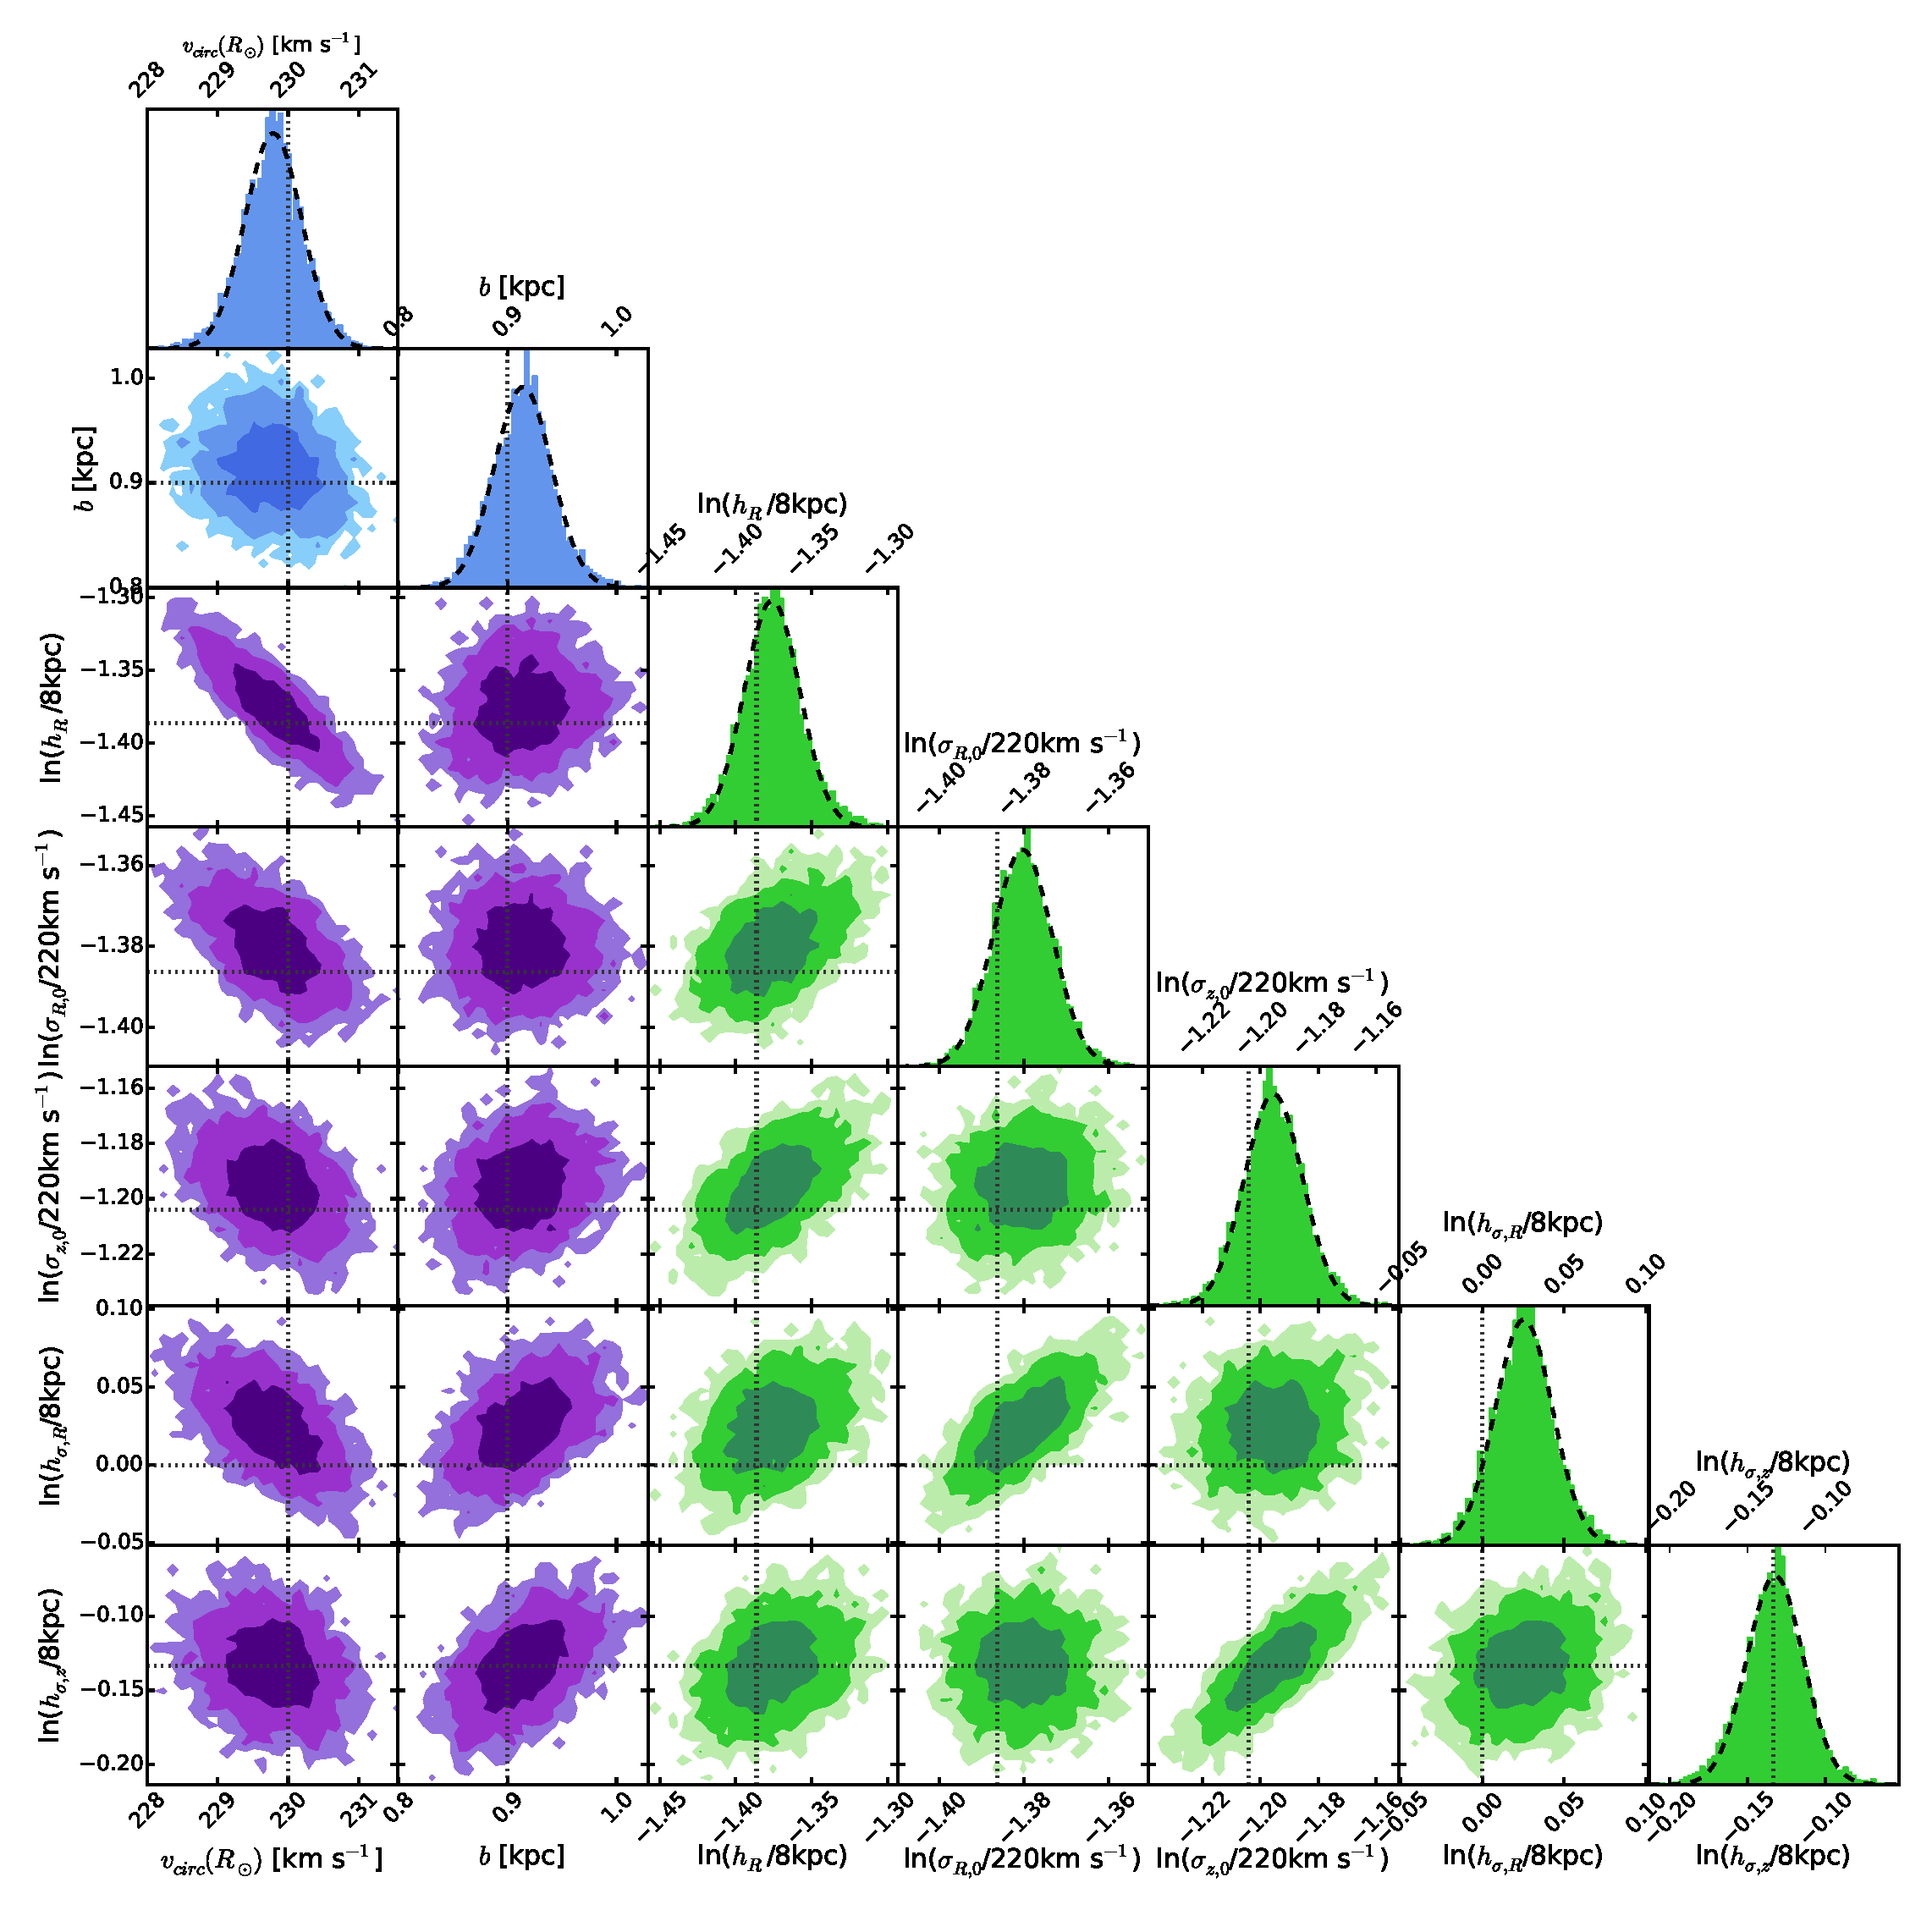
\includegraphics[width=0.7\textwidth]{figs/isoSphFlex_short_hot_2kpc_triangle_MCMC.eps}
%%\plotone{figs/isoSphFlex_short_hot_2kpc_triangle_MCMC.eps}
%\caption{The \pdf{} in the parameter space $\pmodel{} = \{p_\Phi,p_\text{DF}\}$ for one example mock data set created according to Test \ref{test:isoSphFlex} in Table \ref{tbl:tests}. Blue indicates the \pdf{} for the potential parameters, green the qDF parameters. The true parameters are marked by dotted lines. The dark, medium and bright contours in the 2D distributions represent 1, 2 and 3 sigma confidence regions \HW{[TO DO: HW: "likelihood vs. pdf - This is where this matters: is this a confidence on the data or on the parameters?" Don't understand, what he means...]}, respectively, and show weak or moderate covariances. This analysis was picked among five similar analyses, to have all 1 sigma contours encompass the input values \Jo{[TO DO: Jo didn't understand this sentence]}. The \pdf{} here was sampled using MCMC (with flat priors in $p_\Phi$ and  $\ln(p_\text{DF})$ to turn the likelihood in Equation \ref{eq:prob} into a full \pdf{}). Because only 10,000 MCMC samples were used to create the histograms shown, the 2D distribution has noisy contours. The dashed lines in the 1D distributions are Gaussian fits to the histogram of MCMC samples. This demonstrates very well that for such a large number of stars, the \pdf{} approaches the shape of a multi-variate Gaussian, as expected from the central limit theorem \Jo{[TO DO: Jo wrote, that he is not sure if the central limit theorem is directly relevant here]}. \Wilma{[TO DO: rename $h_{\sigma R}$ to $h_{\sigma,R}$, $\sigma_R$ to $\sigma_{R,0}$ and analogous for $z$]}}
%\label{fig:isoSphFlex_triangleplot}
%\end{figure*}
%
%%====================================================================
%
%%FIGURE: width of likelihood propto 1/sqrt(N)
%
%\begin{figure}
%\plotone{figs/sqrtNiso_Stddev_Vs_N.eps}
%\caption{The width of the \pdf{} for two fit parameters found from analyses of 132 mock data sets vs. the number of stars in each data set. The mock data was created in the \texttt{Iso-Pot} potential and all model parameters are given as Test \ref{test:sqrtNiso} in Table \ref{tbl:tests}. The \pdf{} (using the likelihood in Equation \ref{eq:prob} \Wilma{[TO DO: CHECK]}) was evaluated and then a Gaussian was fitted to the marginalized \pdf{} of each free fit parameter. The standard error (SE) of these best fit Gaussians is shown for the potential parameter $b$ in kpc (red dots) and for the qDF parameter $\ln(h_R/8\text{kpc})$ in dimensionless units (blue). The black lines are fits of the functional form SE$(N_\text{sample}) \propto 1/\sqrt{N_\text{sample}}$ to the data points of both shown parameters. As can be seen, for large data samples the width of the \pdf{} behaves as expected and scales with $1/\sqrt{N_\text{sample}}$ as predicted by the central limit theorem. \Wilma{[TO DO: fancybox Legend] [TO DO: write pdf instead of likelihood on y-axis]}} 
%\label{fig:sqrtNiso}
%\end{figure}
%
%%====================================================================
%
%
%%FIGURE: central limit theorem is satisfied
%
%\begin{figure}
%\plotone{figs/isoSph_CLT_2.eps}
%\caption{(Un-)bias of the parameter estimates: According to the central limit theorem the the best fit values for a large number of data sets, each containing a large number of stars, will follow the Normal distribution. To test this, we create 320 mock data sets, which come from two different stellar populations and five spherical observation volumes (see legends). All model parameters are summarized in Table \ref{tbl:tests} as Test \ref{test:isoSph_CLT}. Bias and relative standard error (SE) are derived from the marginalized \pdf{} for one potential parameter (isochrone scale length $b$ in first row) and one qDF parameter ($h_{\sigma,z}$ in second row). The second column displays a histogram of the 320 offsets. As it closely follows a Normal distribution, our modelling method is therefore well-behaved and unbiased. For the 32 analyses belonging to one model we also determine the mean offset and SE, which are overplotted in black in the first two columns (with $1/\sqrt{32}$ as error).  \HW{[TO DO: Is the scatter of the black symbols too large??? Is the reason for this numerical inaccuracies???]} \Wilma{[TO DO: Change test table accordingly, isochrone with b = 1.5 is not used anymore] [TO DO: Caption is too long. Make shorter.] [TO DO: $r_\text{max}$ instead of radius in legend] [TO DO: Leerzeichen fehlt in y-achsenbeschriftung]}}
%\label{fig:isoSph_CLT}
%\end{figure}
%
%%====================================================================

\HW{[TO DO: I sometimes talk about pdf, sometimes about likelihood. We should make this consistent everywhere. I would use \pdf everywhere, but I sometimes reference the likelihood equation. How should I write it in this case?]}